
\documentclass[preprint,12pt]{elsarticle}

\usepackage[spanish]{babel}
\usepackage{amssymb}
\usepackage{graphicx}
\usepackage{lineno}
\usepackage[utf8]{inputenc}
\usepackage{url}
\usepackage{natbib} 
\usepackage{amsmath} 
\usepackage{amssymb} 
\usepackage{float}

\begin{document}
	
	\begin{frontmatter} 

		\title{\huge Informe de Laboratorio Nro 08: Instalación de un Gestor de Base de Datos Oracle}
		
		\author{Estrella Palacios, Katherine Lizbeth         	(2016056193)} 
		\address{Escuela Profesional de Ingeniería de Sistemas}
		\address{Universidad Privada de Tacna}
		\address{Tacna, Perú}
		

	\end{frontmatter}



\section{INFORMACIÓN GENERAL} 

\subsection {\textbf{Objetivos}}
\begin{itemize}
	\item Instalar un Gestor de Base de Datos Oracle
\end{itemize}

\subsection {\textbf{Equipos, materiales, programas y recursos utilizados}}
\begin{itemize}
	\item Computadora con sistema operativo Windows 10.
	\item Min 4GB de RAM
	\item Docker Desktop
	\item Oracle SQL Developer
\end{itemize}


\section{Marco Teórico}



\subsection {\textbf{Docker}}
La palabra "DOCKER" se refiere a varias cosas. Esto incluye un proyecto de la comunidad open source; las herramientas del proyecto open source; Docker Inc., la empresa que es la principal promotora de ese proyecto; y las herramientas que la empresa admite formalmente. El hecho de que las tecnologías y la empresa compartan el mismo nombre puede ser confuso.
\subsubsection{\textbf{Historia}}
Salomon Hykes comenzó Docker comenzó como un proyecto interno dentro de dotCloud,empresa enfocada a PaaS (plataforma como servicio). Fué liberado como código abierto en marzode 2013.Con el lanzamiento de la versión 0.9 (en marzo de 2014) Docker dejó de utilizar LXC comoentorno de ejecución por defecto y lo reemplazó con su propia librería, libcontainer (escrita en Go),que se encarga de hablar directamente con el kernel.Actualmente es uno de los proyectos con más estrellas en GitHub, con miles debifurcaciones (forks) y miles de colaboradores.

\subsubsection{\textbf{Características}}
Las principales características de Docker son:


\begin{itemize}
\item \textbf{Portabilidad:} el contenedor Docker podemos desplegarlo en cualquier sistema, sin necesidad de volver a configurarlo o realizar las instalaciones necesarias para que la aplicación funcione, ya que todas las dependencias son empaquetadas con la aplicación en el contenedor.

\item \textbf{Ligereza:} los contenedores Docker sólo contienen lo que las diferencia del sistema operativo en el que se ejecutan, no se virtualiza un SO completo.

\item \textbf{Autosuficiencia:} un contenedor Docker no contiene todo un sistema operativo completo,sólo aquellas librerías, archivos y configuraciones necesarias para desplegar las funcionalidades que contenga.
\end{itemize}


\subsection{\textbf{Oracle}}
Oracle la Primera Base de Datos Diseñada para Grid Computing, es un sistema de gestión de base de datos relacional fabricado por Oracle Corporation.
Oracle es básicamente un herramienta cliente/servidor para la gestión de base de datos la gran potencia que tiene y su elevado precio hace que solo se vea en empresas muy grandes y multinacionales, por norma general.
Oracle Corporation :es una de las mayores compañías de software del mundo. Sus productos van desde bases de datos (Oracle) hasta sistemas de gestión. Cuenta además, con herramientas propias de desarrollo para realizar potentes aplicaciones, como Oracle Designer
\subsubsection{\textbf{Historia}}
Oracle surge a finales el año 1970 del nombre de Relational Software a partir de un estudio sobre SGBD (Sistemas Gestores de Base de Datos) Computer World definió este estudio como uno de los más completos jamás escritos sobre bases de datos.
usaba la filosofía de las bases de datos relacionales, algo que por aquella época era todavía desconocido.
La tecnología Oracle se encuentra prácticamente en todas las industrias alrededor del mundo.
Oracle es la primera compañía de software que desarrolla e implementa software para empresas 100 por ciento activado por Internet a través de toda su línea de productos: base de datos, aplicaciones comerciales y herramientas de desarrollo de aplicaciones y soporte de decisiones.
Oracle garantiza el funcionamiento de sus bases de datos, que en caso de caidas del servidor compensa economicamente con cifras cercanas a las 7 cifras. 

\subsubsection{\textbf{Características}}
Desarrollado sobre Oracle Database, Oracle Content Database ha sido diseñada para que las organizaciones puedan controlar y gestionar grandes volúmenes de contenidos no estructurados en un único repositorio con el objetivo de reducir los costes y los riesgos asociados a la pérdida de información. 

\subsubsection{\textbf{Estructura}}
Una BD Oracle tiene una estructura física y una estructura lógica : 
\begin{itemize}
	\item La estructura física se corresponde a los ficheros del sistema operativo.
	\item La estructura lógica está formada por los tablespace y los objetos de un esquema de BD 
\end{itemize}


\section{PROCEDIMIENTO}

\subsubsection{\textbf{Paso 1: Ingresar a Docker Setup}}
\begin{figure}[H]
	\begin{center}
		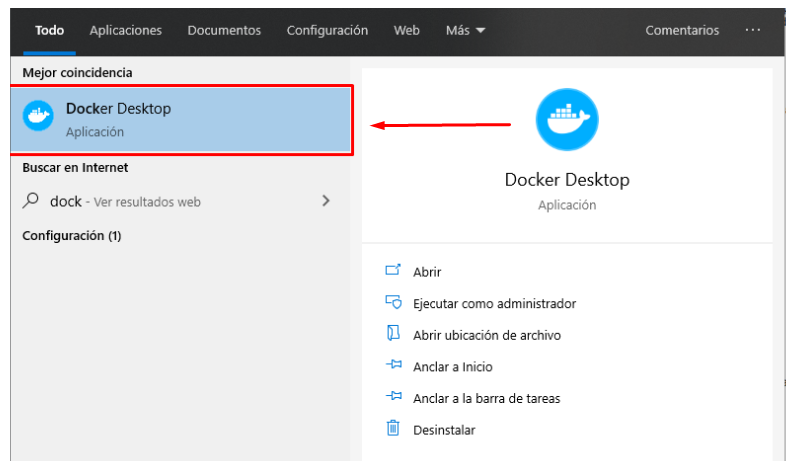
\includegraphics[width=12cm]{./IMAGENES/foto1} 
	\end{center}
\end{figure}

\begin{figure}[H]
	\begin{center}
		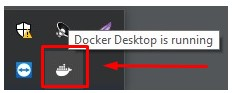
\includegraphics[width=12cm]{./IMAGENES/foto2} 
		\caption{Docker se encuentra en ejecucion}
	\end{center}
\end{figure}

\begin{figure}[H]
	\begin{center}
		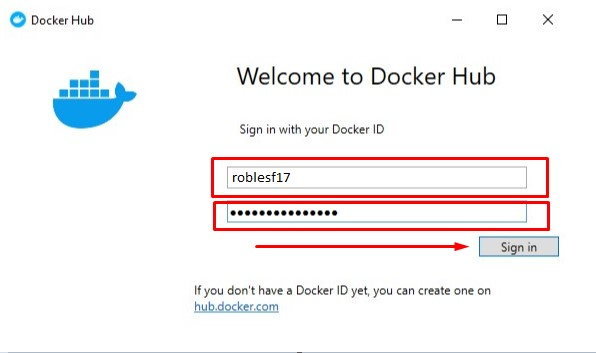
\includegraphics[width=12cm]{./IMAGENES/foto3} 
		\caption{Iingresar la cuenta Docker}
	\end{center}
\end{figure}

\begin{figure}[H]
	\begin{center}
		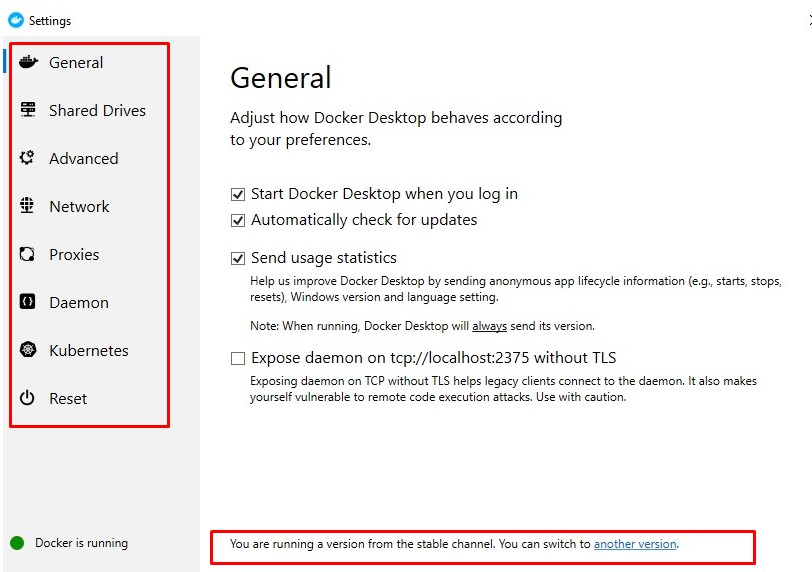
\includegraphics[width=12cm]{./IMAGENES/foto4} 
		\caption{Ventana principal de Docker}
	\end{center}
\end{figure}

\subsubsection{\textbf{Paso 2: Utilizaremos PowerShell para gestionar}}

\begin{figure}[H]
	\begin{center}
		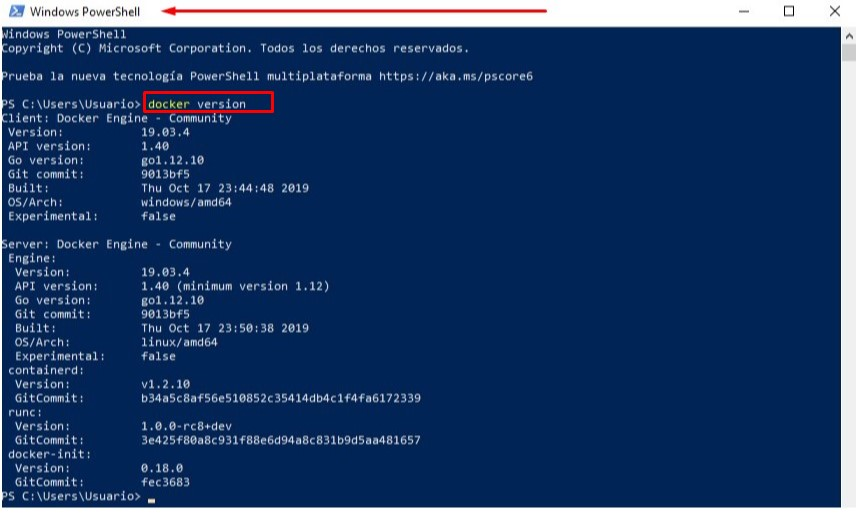
\includegraphics[width=12cm]{./IMAGENES/foto5} 
		\caption{“Docker versión” para confirmar la instalacion de Docker}
	\end{center}
\end{figure}


\begin{figure}[H]
	\begin{center}
		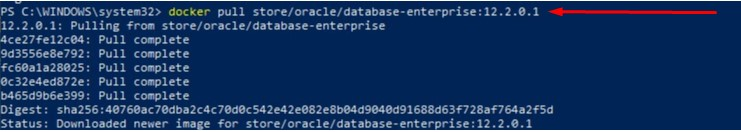
\includegraphics[width=12cm]{./IMAGENES/foto6} 
		\caption{Descargamos la iso}
	\end{center}
\end{figure}

\begin{figure}[H]
	\begin{center}
		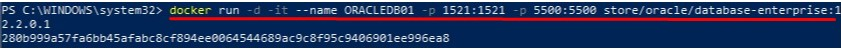
\includegraphics[width=12cm]{./IMAGENES/foto10} 
		\caption{Instalamos el contenedor}
	\end{center}
\end{figure}

\begin{figure}[H]
	\begin{center}
		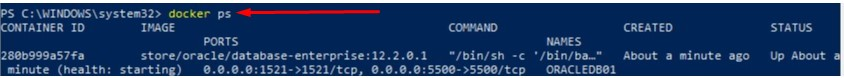
\includegraphics[width=12cm]{./IMAGENES/foto11} 
		\caption{Verificamos se instalo correctamente}
	\end{center}
\end{figure}

\subsubsection{\textbf{Paso 3: Ejecutar}}
\begin{figure}[H]
	\begin{center}
		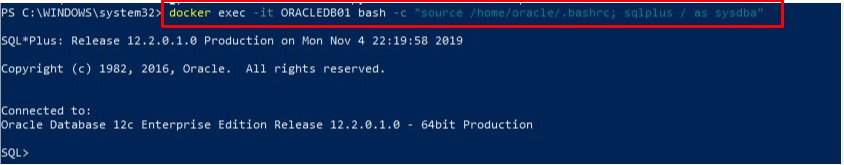
\includegraphics[width=12cm]{./IMAGENES/foto12} 
		\caption{Ejecutaremos el docker}
	\end{center}
\end{figure}

\begin{figure}[H]
	\begin{center}
		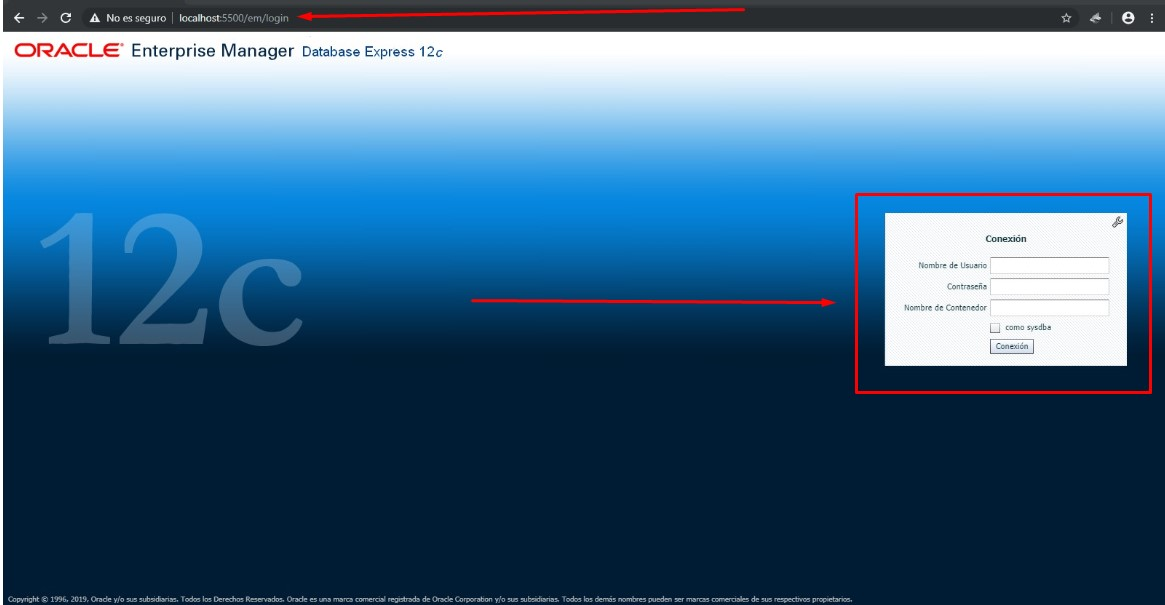
\includegraphics[width=12cm]{./IMAGENES/foto13} 
		\caption{Conectemos a la base de datos creadas}
	\end{center}
\end{figure}

\begin{figure}[H]
	\begin{center}
		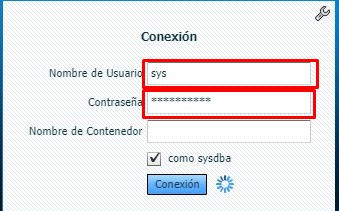
\includegraphics[width=12cm]{./IMAGENES/foto14} 
		\caption{Accederemos de la forma predeterminada}
	\end{center}
\end{figure}

\begin{figure}[H]
	\begin{center}
		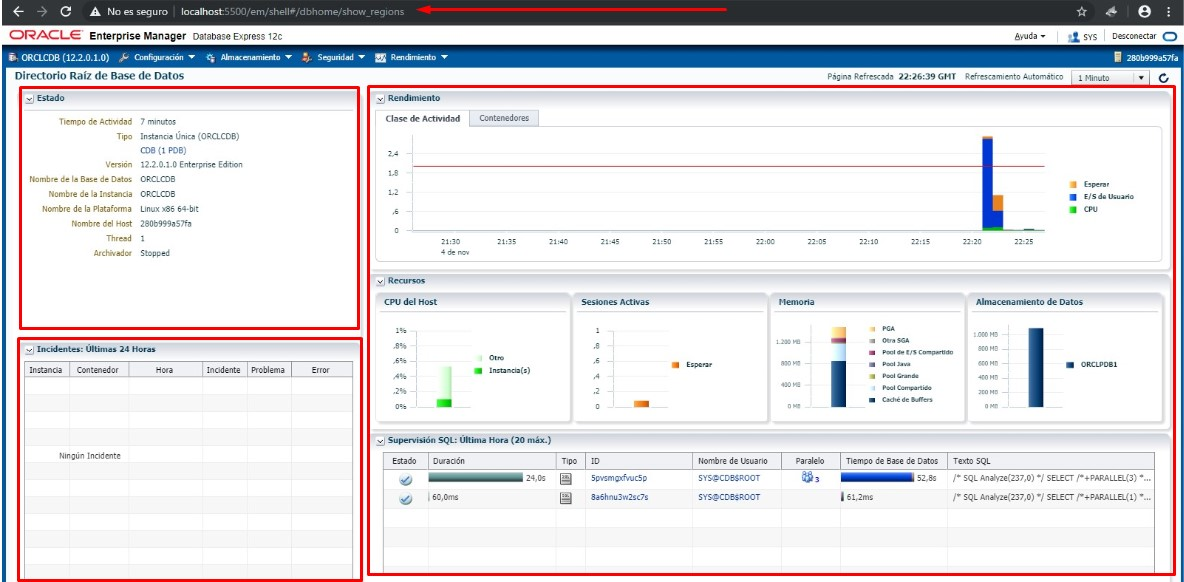
\includegraphics[width=13cm]{./IMAGENES/foto15} 
		\caption{Interfaz grafica principal de ORACLE}
	\end{center}
\end{figure}


\section{ANALISIS E INTERPRETACION DE RESULTADOS }
\begin{itemize}
	\item ¿Qué indican los resultados? \\
	Se reaclizo exitosamente la conexion con el contenedor de base de datos.
	\item ¿Que se ha encontrado?\\
	Tener una base de datos Oracler sin necesidad de estar haciendo toda la instalación necesaria en el computador.
\end{itemize}


\section{CONCLUSION}
Docker es una herramienta de código abierto que desde hace ya algunos años se está hablando mucho y cada vez más. Con Docker podremos ejecutar un conjunto de procesos de forma aislada, crear herramientas gracias a sus imágenes y compartirlas gracias al repositorio que tienen.

\end{document}
